\documentclass[12pt]{article}
\usepackage[utf8]{inputenc}
\usepackage{graphicx}
\usepackage{tikz}
\usepackage{verbatim}
\usepackage{amsmath}
\usepackage{amsfonts}
\usepackage{amssymb}
\usepackage{hyperref}
\usepackage{natbib}

\usepackage{lettrine}  % Enables drop caps


\usepackage{listings}
\usepackage{xcolor}  % for custom colors
\usepackage{float}
\usepackage{enumitem}


\renewcommand{\today}{\ifcase\month \or January\or February\or March\or April\or May\or June\or July\or August\or September\or October, \or November\or December\fi \number\year} 

\lstset{
  basicstyle=\ttfamily,
  columns=fullflexible,
  frame=single,
  breaklines=true,
  postbreak=\mbox{\textcolor{red}{$\hookrightarrow$}\space},
  commentstyle=\color{gray},
  keywordstyle=\color{blue},
  stringstyle=\color{red},
  numbers=left,
  numberstyle=\tiny,
  numbersep=5pt,
  escapeinside={(*@}{@*)}
}

\title{
University Of Oslo\\ 
\large FYS2150\\
\large Solar Cell\\}
\author{Raji Youssef}
\date{}


\begin{document}
\maketitle

\begin{abstract}
\lettrine[lines=1]{T}{his} project examines the behavior  of solar cells under both uniform and non-uniform illumination conditions. The goal is to understand how solar cells can be practically used as sources of electrical power.

We first identify a single solar cell by measuring its current–voltage (I–V) curve in both dark and illuminated conditions . We then study how the power output varies with different resistances and when the cell produces the maximum power. We found that the power increases as we increase the load up to a certain point, after which it begins to decrease.

Next, two identical cells are connected in series and in parallel, and we compare their efficiency. In the final part, one of the cells is partially shaded to simulate  conditions in reality  where solar cells can be exposed to uneven light. We found that parallel-connected solar cells are more efficient than series-connected ones under different conditions.  




\end{abstract}
\section{Introduction }
Extracting energy is one of the greatest challenges of our time. The demand for a low-cost and efficient energy source that does not harm the planet is currently a major challenge for our race .

Solar energy is one of the most accessible and sustainable energy sources available to us today. The sun is the main source of external energy that we receive on our  planet, and it powers a large number of the planet's natural phenomena  that can be used for our benefit  . This makes the  conversion of sunlight into electrical energy  an interesting  subject, 

A solar cell is a semiconductor device that converts  light into electrical energy based on  the photoelectric effect. When photons with enough energy shines on  the surface of the cell, they  excite electrons causing them to be ejected from their atoms , running a current in an  circuit. The efficiency of this process depends on several factors, including the wavelength of the  light, the intensity of illumination, and the electrical load connected to the cell as well as how cells are connected together. 

In this series of experiments, we will focus on the effect of resistance variation on the power delivered  by a single cell. We will also study  two types of connecting solar cells : series connecting and parallel connecting and compare their efficiency in both uniform and non-uniform light.   
 

\section{theory }
The solar cells are made of a semiconductor material . 
A semiconductor is a material with electrical conductivity between that of a conductor and an insulator  commonly based on silicon. . 
Silicon atoms have four valence electrons and form a crystal  by sharing electrons with neighboring atoms, satisfying the 8-rule  and creating strong bonds.
When an  electron gains enough energy, it can escape the bond and become a free electron, leaving behind a vacancy known as a "hole" needs to be filled .An electron from a neighboring atom will jump to fill this hole, creating a new hole in its original location . This causes both electrons and holes to move through the crystal, with holes  moving in the opposite direction to the electrons. The more electrons that are released and holes that are created, the better is  the conductivity.

To further improve conductivity, a process known as  "doping "is used. This process is based on  replacing approximately one in \textbf{\( 10^6 \)}
silicon atoms with atoms of a different element.That allows us to improve conductivity without affecting the structure of the crystal. 
  
Doping with atoms that have five valence electrons gives extra free electrons and creates an n-type semiconductor .Doping with atoms that have three valence electrons  increases the number of holes and creates  a p-type semiconductor.
In solar cells a combination of these two types of semiconductor is used and it is called "pn-junction "  as shown in the figure \ref{fig:1} below:

\begin{figure}[hbt!]
    \center
    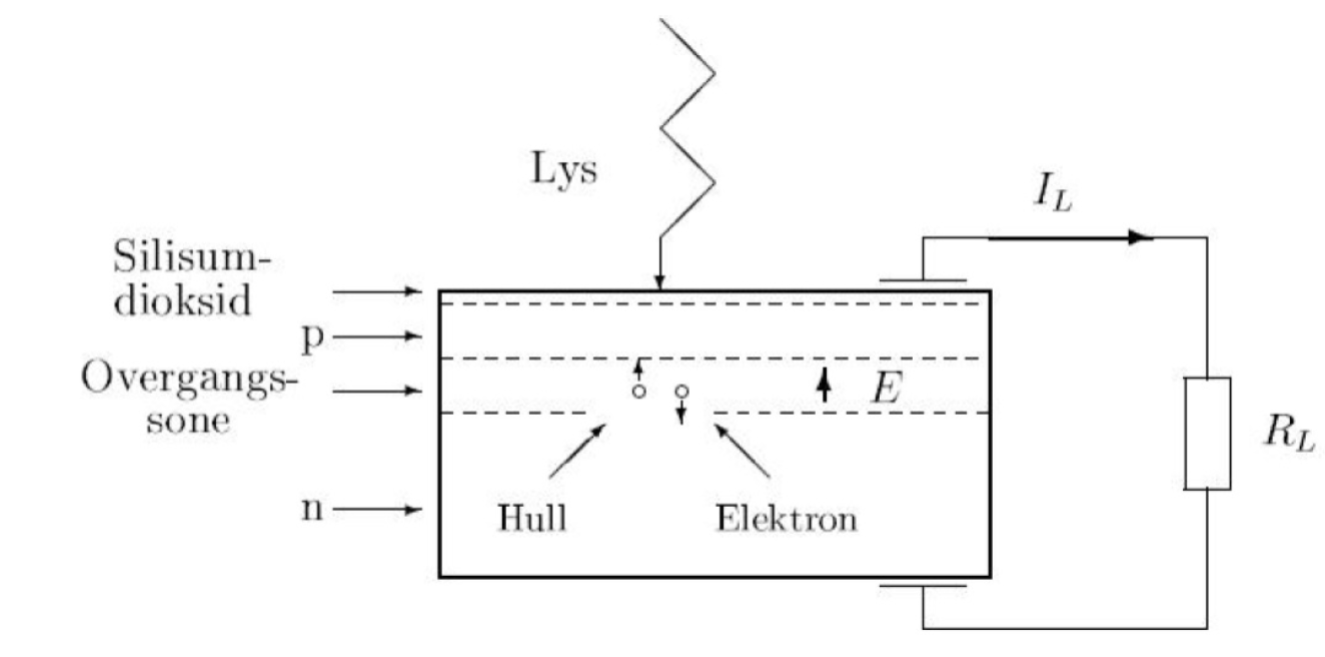
\includegraphics[scale=0.5]{1.png}
\caption{ Solar cell as semiconductor}
\label{fig:1}
\end{figure}

In the region between the p-side and n-side (called the transition area), there exists an electric field directed from the n-side to the p-side. This field prevents further movement of charges from the n-region to the p-region.
\newline

In the absence of light, a solar cell behaves like a standard p–n junction. However, the situation changes when light with enough energy shines on the junction. Light striking the transition region will release bound electrons, creating free electrons and hence holes .The internal electric field then drives the electrons toward the n-region and the holes toward the p-region.
\newline

As a result, electrons gather  in the n-region and holes in the p-region, a potential difference (voltage) is created across the junction, with the p-side becoming positively charged and the n-side negatively charged.
Over time, the field in the transition zone decreases, and the flow of charge   stops. To keep a continuous flow, a  conductor is externally connected between the p- and n-regions. This allows electrons to continue  flowing from the n-side to the p-side through the wire, producing an  current in the circuit . The current will remain as long as light continues to reach the solar cell.
\newline

In our discussion, We will only be using formulas related to voltage, current, and resistance. Therefore, \textbf{ Ohm's law }is useful to our analysis : 
\begin{equation}
I = \frac{V}{R}
\label{eq:v/r}
\end{equation}
Where :
\begin{itemize}
    \item \( V \): Is the voltage  .
    \item \( R \): is the resistance . 
    \item \( I \): is the current .
\end{itemize}

To study the effect delivered by the solar cell , we also use the formula for\textbf{ electrical power} : 
\begin{equation}
P = IV =  \frac{V^2}{R}
\label{eq:IV}
\end{equation}
where :
\begin{itemize}
    \item \( V \): Is the voltage  .
    \item \( R \): is the resistance . 
    \item \( I \): is the current .
    \item \( P \): is the effect delivered by the solar cell.
\end{itemize}




\section{Experimentally}

In the following  series of experiments ,we will use these equipments :
\begin{itemize}
    \item A light projector.
    \item A voltage source.
    \item Two multimeter.
    \item A selection of resistors.
    \item Two identical solar cells.
    \item connecting wires.
\end{itemize}

\subsection{Uncertainty Analysis}
\textbf{Instruments uncertainties:}\cite{manual}

\begin{itemize}
    \item Voltage (\( V \)): measured using a digital multimeter with an uncertainty of \( \pm 0.025 \%  \) of the reading in V.
    \item Current (\( I \)): measured using a digital Ammeter with an uncertainty of \( \pm 0.05\%  \) of the reading .
    \item Resistance (\( R \)): assumed uncertainty of \( \pm 0.05\% \) of the reading in (\( \Omega \))  for the variable resistor
\end{itemize}


\textbf{Uncertainty in power calculation :}

The power  \( P \) is calculated using the formula:
\[
P = I \cdot V
\]

To calculate the uncertainty in power \( \Delta P \), we use the standard formula of uncertainty for multiplication \cite{squires}:
\begin{equation}
\frac{\Delta P}{P} = \frac{\Delta I}{I} + \frac{\Delta V}{V} \\
\Rightarrow \quad
\Delta P = P \left( \frac{\Delta I}{I} + \frac{\Delta V}{V} \right)
\label{eq:delta P}
\end{equation}




\subsection{Solar cell as a semiconductor}
The purpose of this experiment is to examine the difference in the behavior of a solar cell when exposed to light compared to when it is in darkness.
\newline

We begin by setting up the experiment using a one solar cell. A multimeter is connected in parallel to measure the voltage,  an ammeter is connected in series to measure the current. A resistor is included in the setup, and the whole circuit  is connected to a power supply, as shown in figure  \ref{fig:2}:

\begin{figure}[H]
    \center
    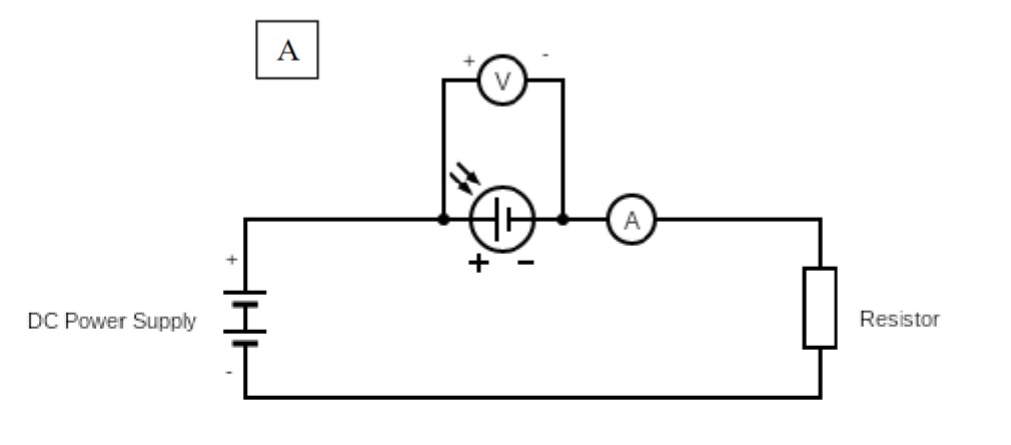
\includegraphics[width=\linewidth]{2.png}
\caption{ Setup for measuring solar cell current-voltage characteristics}
\label{fig:2}
\end{figure}

The experiment will be repeated in two different situations:    
\begin{itemize}
    \item  Part A: When the solar cell is exposed to light  .
    \item  Part B: :When the solar cell is in darkness. 
\end{itemize}


The ammeter is set to a value of \(300 \)mA and a resistance of \( 10\Omega \).

First, we performed measurements in the absence of light,where we recorded the current I and voltage V over a  voltage ranging \( -5 \)V to\( +5 \)V  in increments of  \( 0.25 \)V.

Next, we repeated the experiment under illumination by placing the solar cell in front of  a desk lamp located at at  distance \( 50 \)cm  as shown  in figure \ref{fig:3}: 
\begin{figure}[H]
    \center
    \includegraphics[width=\linewidth]{Opsett.jpg}
\caption{ A solar cell illuminated by a light source }
\label{fig:3}
\end{figure}

 Current and voltage were measured over the same voltage range. 
Once all the measurements were obtained,  we plotted them against each other to obtain the characteristic  curve and  compare it  to the theoretical reference curve shown in figure \ref{fig:4}  below:

\begin{figure}[H]
    \center
    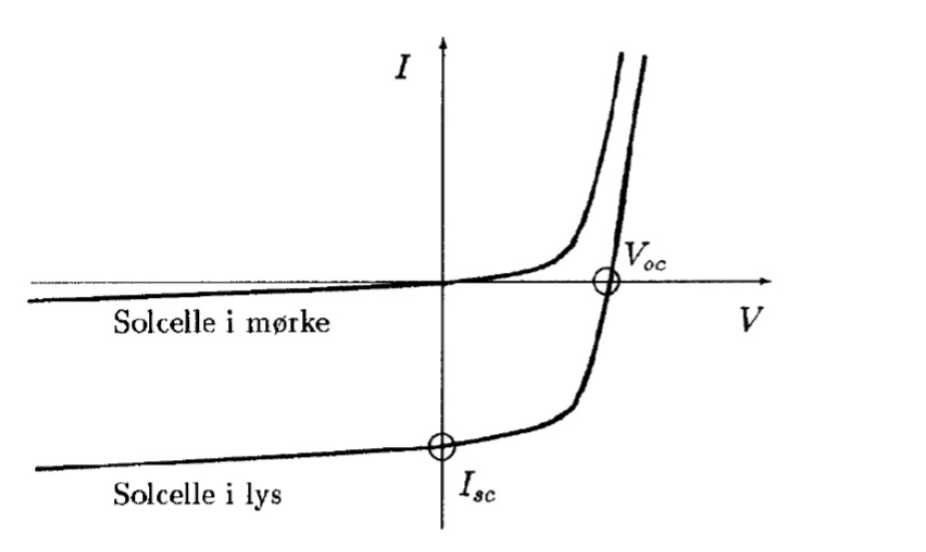
\includegraphics[width=\linewidth]{3.png}
\caption{ The theoretical IV
curve for a solar cell in light vs in darkness}
\label{fig:4}
\end{figure}

\subsection{The Solar Cell's Optimal Load}

This experiment consists of two solar cells placed in front of a projector lamp. In the first part, only one cell will be used. The cell should be placed in front of the lamp in such a way that a second cell can be added later without moving the first one.

In \textbf{Part A}, we will measure the current and voltage produced by the solar cell, without using an external voltage source or resistance.

In \textbf{Part B}, a variable resistor will be added to the circuit. The resistance will range from \(  0.2\Omega\)to  \(10 \Omega  \).

The aim here is to use as few connecting  cables as possible to minimize  uncertainty in \textbf{R}

Finally,  the effect can be computed using the formula \eqref{eq:IV}.
We then use our measurements to plot the electrical power \textbf{P} as a function of the resistance \textbf{R} in the circuit to find  the value of R when the cell was the most efficient .

\subsection{Combination of single solar cells into a solar panel}
In this assignment, we examine solar cells connected in series and parallel configurations. Both types of configurations are often used in solar panel systems, and our goal is to investigate the advantages and disadvantages  of each.

We will analyze each configuration separately as shown in the figures \ref{fig:5} and \ref{fig:6}   below : 

\begin{figure}[H]
    \center
    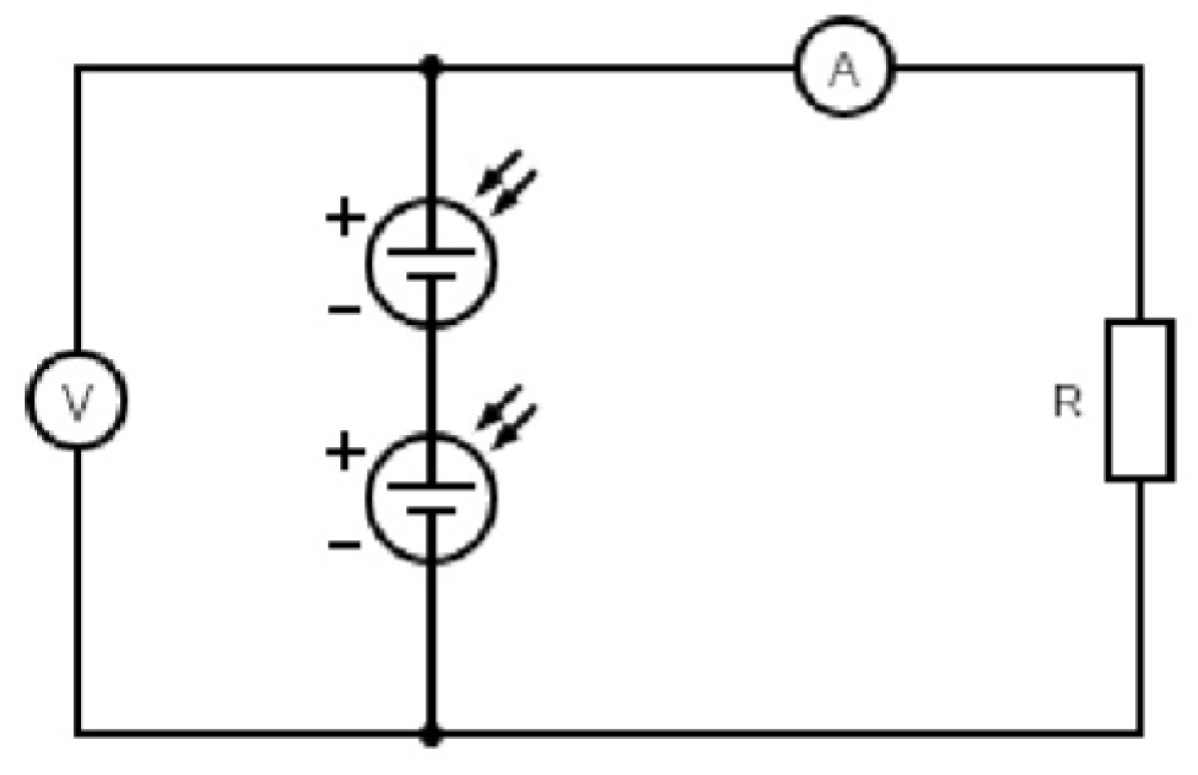
\includegraphics[width=\linewidth]{5.png}
\caption{ Two identical solar cells connected in series}
\label{fig:5}
\end{figure}

\begin{figure}[H]
    \center
    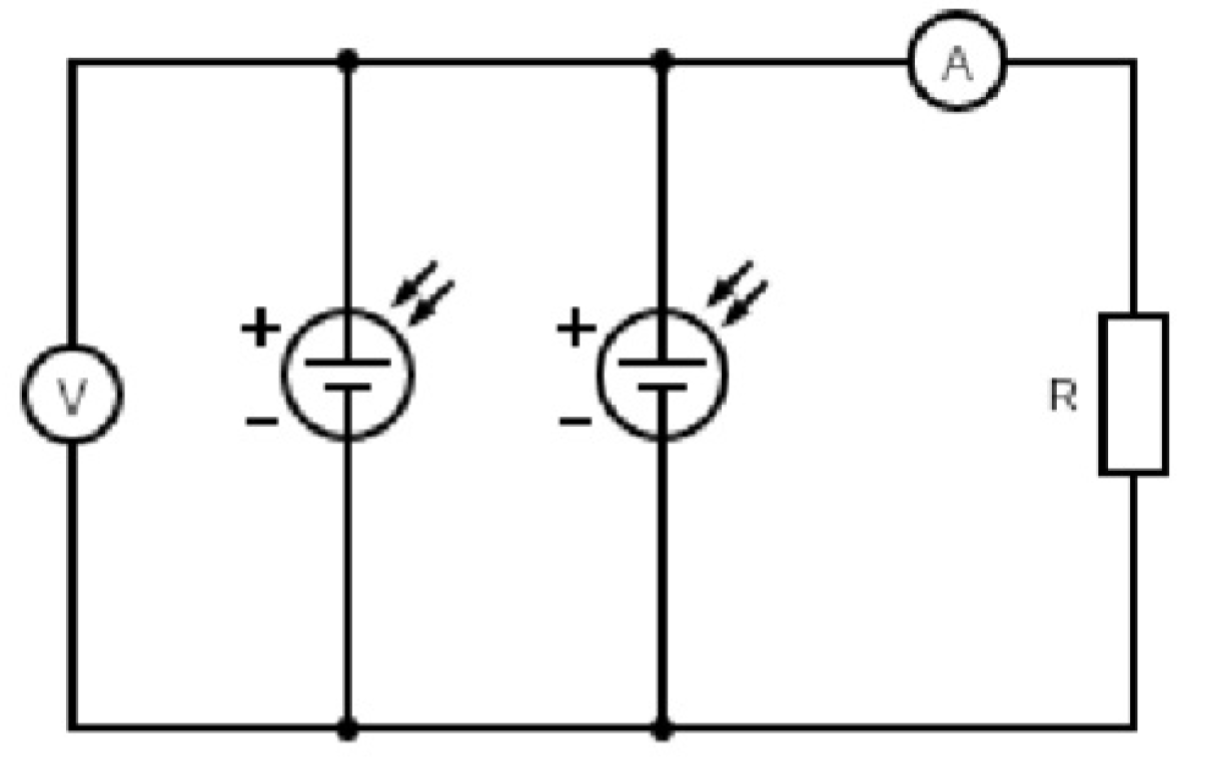
\includegraphics[width=\linewidth]{6.png}
\caption{ Two identical solar cells connected in parallel}
\label{fig:6}
\end{figure}
First,  we will be take measurements for both setups under full illumination.
Our goal is  to determine the maximum power  can be produced  in each case.

\textbf{In part A} ,we will measure the behavior  of solar cells connected in series. The cells will be placed at equal distances from the light source, and we will record current and voltage measurements for different values of resistances.Then,we will plot effect \textbf{P} 
as a function of  resistance \textbf{R}.

\textbf{In part B} , we will repeat the same process using parallel-connected solar cells.

\subsection{Non-Uniformly illumination}

In this experiment, we will examine series-connected and parallel-connected solar cells, with a difference being that we will change the illumination condition .

In real-world scenario such as installing multiple solar cells on the roof of a house or cabin ,the lighting  often not even . Roofs may be partially shaded by trees, clouds etc. In this experiment, we will  study the effect of partial shading on power production  and optimal load for different connection types.

To visualize  this case, we will place one of the solar cells in  shadow by placing an object between it and the  light source, while keeping the other cell   illuminated.
This setup will be repeated for both series-connected and parallel-connected solar cells.

Again, we will measure the current and voltage for different \textbf{R} values, calculate the power  
P, and plot it as a function of resistance \textbf{R} for both cases and compare which connection type generates a better effect under different illumination conditions



Again, we will plot the power output \textbf{P} as function of  resistance \textbf{R} for both cases and compare which connection type generates the better effect in none-uniformly lightning.

\section{Results}
\subsection{Solar cell as a semiconductor}
\textbf{Part A: When the solar cell is exposed to light:}
We performed the experiment and obtained the results shown in the table \ref{tab:light_measurements}:
\begin{table}[H]
\centering
\begin{tabular}{|c|c|}
\hline
\textbf{I\textsubscript{light} \( \pm0.05\% \) (mA)} & \textbf{V\textsubscript{light} \( \pm0.025\% \)(V)} \\
\hline
126.4  & 0.52  \\
93.9   & 0.51  \\
74.6   & 0.50  \\
58.8   & 0.49  \\
26.63  & 0.47  \\
-1.72  & 0.44  \\
-25.34 & 0.40  \\
-35.0  & 0.37  \\
-39.4  & 0.35  \\
-43.5  & 0.30  \\
-47.7  & 0.24  \\
-49.1  & 0.21  \\
-50.5  & 0.15  \\
-51.1  & 0.11  \\
-51.6  & 0.05  \\
-52.5  & -0.49 \\
-52.7  & -1.00 \\
-53.8  & -1.93 \\
-55.8  & -3.04 \\
-58.1  & -3.94 \\
\hline
\end{tabular}
\caption{Measured current and voltage values for a single solar cell under illumination.}
\label{tab:light_measurements}
\end{table}

\textbf{Part B: :When the solar cell is in darkness:}

We performed the experiment and obtained the results shown in the table \ref{tab:dark_measurements}:

\begin{table}[H]
\centering
\begin{tabular}{|c|c|}
\hline
\textbf{I\textsubscript{dark}\(\pm0.05\%\) (mA)} & \textbf{V\textsubscript{dark}\(\pm0.025\%\) (V)} \\
\hline
97.8   & 0.503  \\
61.4   & 0.475  \\
43.8   & 0.453  \\
27.66  & 0.421  \\
23.90  & 0.411  \\
13.08  & 0.361  \\
12.46  & 0.357  \\
8.00   & 0.319  \\
6.27   & 0.298  \\
4.85   & 0.277  \\
3.72   & 0.257  \\
2.45   & 0.227  \\
1.56   & 0.199  \\
0.92   & 0.170  \\
-0.24  & 0.000  \\
-0.21  & -0.25  \\
-0.35  & -0.42  \\
-0.66  & -0.77  \\
-1.01  & -1.00  \\
-1.20  & -1.26  \\
-1.47  & -1.49  \\
-1.84  & -1.77  \\
-2.17  & -2.00  \\
-2.52  & -2.25  \\
-3.01  & -2.55  \\
-3.28  & -2.71  \\
-3.78  & -2.98  \\
-4.56  & -3.34  \\
-5.32  & -3.54  \\
-5.77  & -3.77  \\
-6.36  & -3.97  \\
-7.21  & -4.27  \\
-7.76  & -4.62  \\
-8.78  & -4.75  \\
-9.57  & -4.98  \\
\hline
\end{tabular}
\caption{Measured current and voltage values for a single solar cell in darkness.}
\label{tab:dark_measurements}
\end{table}
Plugging the values from both tables into a Python program and plotting the results against each others , we obtained the following IV curve shown in the figure  \ref{fig:7}:

\begin{figure}[h]
    \center
    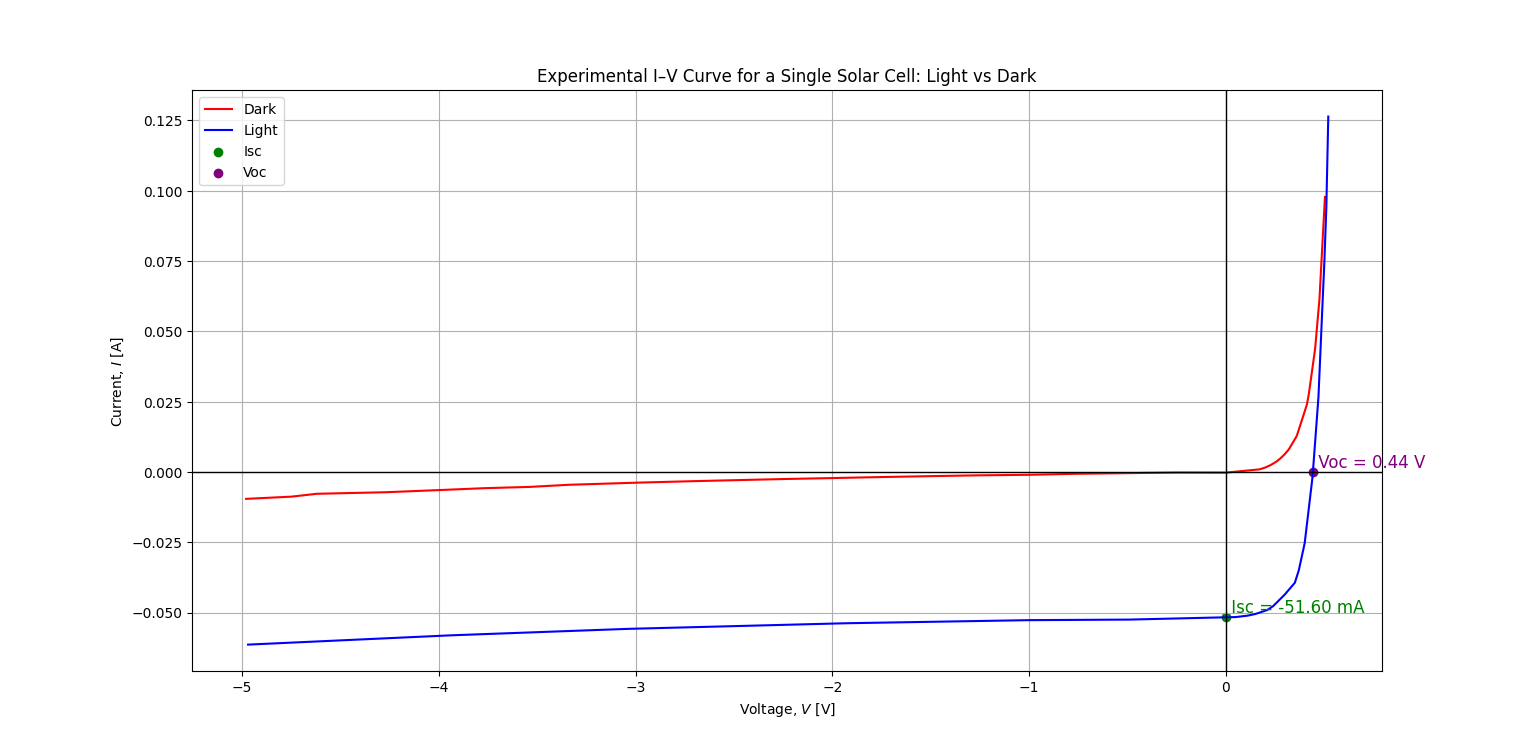
\includegraphics[width=\linewidth]{7.png}
\caption{ The experimental IV
curve for a single  solar cell in light vs in darkness , also showing the intersecting points  }
\label{fig:7}
\end{figure}
The intersecting points with I and V  were calculated to be : 
\(V_{oc} = 0.44  \)V , \(I_{sc} = 51.6  \)mA.

\subsection{The Solar Cell's Optimal Load}
\textbf{Part A : measuring the current and voltage produced by the solar cell, without using an external voltage source or resistance.} 
\newline
The resistance in Ammeter was \(0.2-0.3 \Omega  \).
\newline

First , we measure the highest value for I and V individually without  resistance:
\begin{itemize}
    \item  \(I_{max}  = 0.14 \pm 0.007 \)A.
    \item  \(V_{max}  = 0.496\pm 0.01 \)V. 
\end{itemize}

Next , we measure the highest value for I and V simultaneously to be : 

\begin{itemize}
    \item  \(I_{max}  = 0.141 \pm 0.007 \)A.
    \item  \(V_{max}  = 0.009 \pm 0.01 \)V. 
\end{itemize}

\textbf{Part B: measuring the voltage and the current produced by solar cells with a variable resistance:}
The experiment was performed using different values of resistance R, and recorded the  voltage and current measurements  . The results are shown in the table \ref{tab:variable_resistance}   below:

\begin{table}[H]
\centering
\begin{tabular}{|c|c|c|}
\hline
\textbf{I \(\pm0.05\%\)(mA)} & \textbf{V \(\pm0.025\%\)(V)} & \textbf{R \(\pm0.05\%\)($\Omega$)} \\
\hline
0.14  & 0.015 & 0.0  \\
0.139 & 0.043 & 0.2  \\
0.139 & 0.071 & 0.4  \\
0.14  & 0.099 & 0.6  \\
0.139 & 0.126 & 0.8  \\
0.139 & 0.149 & 1.0  \\
0.138 & 0.176 & 1.2  \\
0.137 & 0.203 & 1.4  \\
0.137 & 0.215 & 1.5  \\
0.136 & 0.229 & 1.6  \\
0.136 & 0.240 & 1.7  \\
0.135 & 0.253 & 1.8  \\
0.134 & 0.265 & 1.9  \\
0.133 & 0.276 & 2.0  \\
0.128 & 0.329 & 2.5  \\
0.12  & 0.373 & 3.0  \\
0.119 & 0.376 & 3.1  \\
0.117 & 0.384 & 3.2  \\
0.115 & 0.389 & 3.3  \\
0.113 & 0.394 & 3.4  \\
0.111 & 0.400 & 3.5  \\
0.103 & 0.417 & 4.0  \\
\hline
\end{tabular}
\caption{Measured current, voltage, and resistance values for a solar cell with variable resistance.}
\label{tab:variable_resistance}
\end{table}
The corresponding P-R curve was obtained by inserting the values in the table \ref{tab:variable_resistance} into a Python code as shown in figure \ref{fig:8}:

\begin{figure}[H]
    \center
    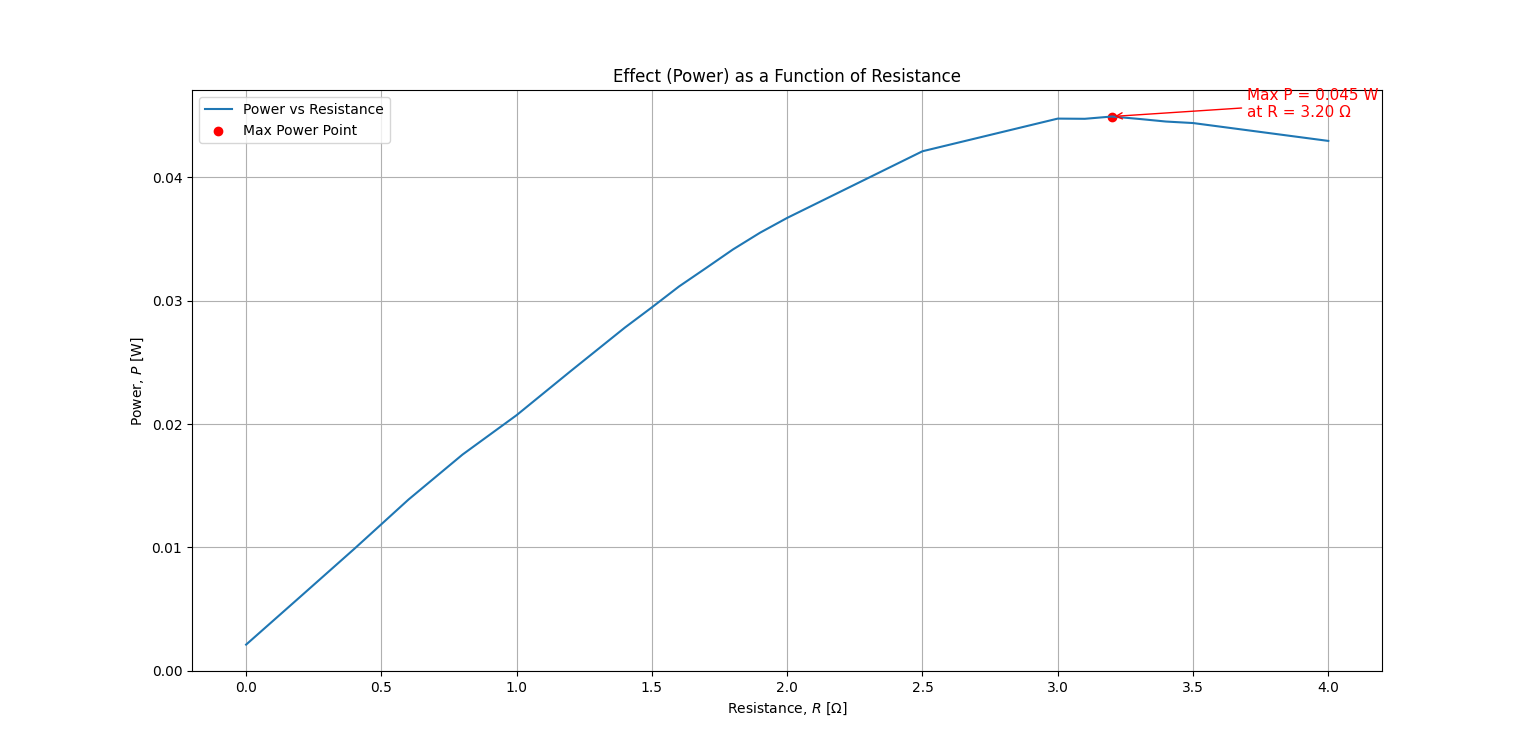
\includegraphics[width=\linewidth]{8.png}
\caption{ The P-R curve  showing the  effect as a function of resistance  }
\label{fig:8}
\end{figure}
As shown in the plot , the maximum value of P :  \( P_{max} = 0.043 \pm0.0055 \) W corresponds to the resistance \( R = 3.2 \pm0.16 \Omega \).
\subsection{Combination of single solar cells into a solar panel}
\textbf{Part A} : solar cells connected in
series. The measurements obtained for  this configuration are shown in the table \ref{tab:cell_series}

\begin{table}[H]
\centering
\begin{tabular}{|c|c|c|}
\hline
\textbf{I\(\pm0.05\%\) (mA)} & \textbf{V\(\pm0.025\%\) (V)} & \textbf{R\(\pm0.05\%\) ($\Omega$)} \\
\hline
0.123 & 0.014 & 0.0  \\
0.122 & 0.131 & 1.0  \\
0.123 & 0.256 & 2.0  \\
0.124 & 0.317 & 2.5  \\
0.123 & 0.378 & 3.0  \\
0.123 & 0.504 & 4.0  \\
0.120 & 0.610 & 5.0  \\
0.117 & 0.709 & 6.0  \\
0.113 & 0.745 & 6.5  \\
0.112 & 0.752 & 6.6  \\
0.112 & 0.758 & 6.7  \\
0.111 & 0.765 & 6.8  \\
0.110 & 0.771 & 6.9  \\
0.110 & 0.779 & 7.0  \\
0.109 & 0.784 & 7.1  \\
0.108 & 0.789 & 7.2  \\
0.107 & 0.793 & 7.3  \\
0.107 & 0.799 & 7.4  \\
0.106 & 0.805 & 7.5  \\
0.102 & 0.827 & 8.0  \\
\hline
\end{tabular}
\caption{Measured current, voltage, and resistance values for a solar cell connected in series .}
\label{tab:cell_series}
\end{table}

Plotting these values to obtain the P-R curve for series connected solar cells as shown in figure  \ref{fig:9}:

\begin{figure}[H]
    \center
    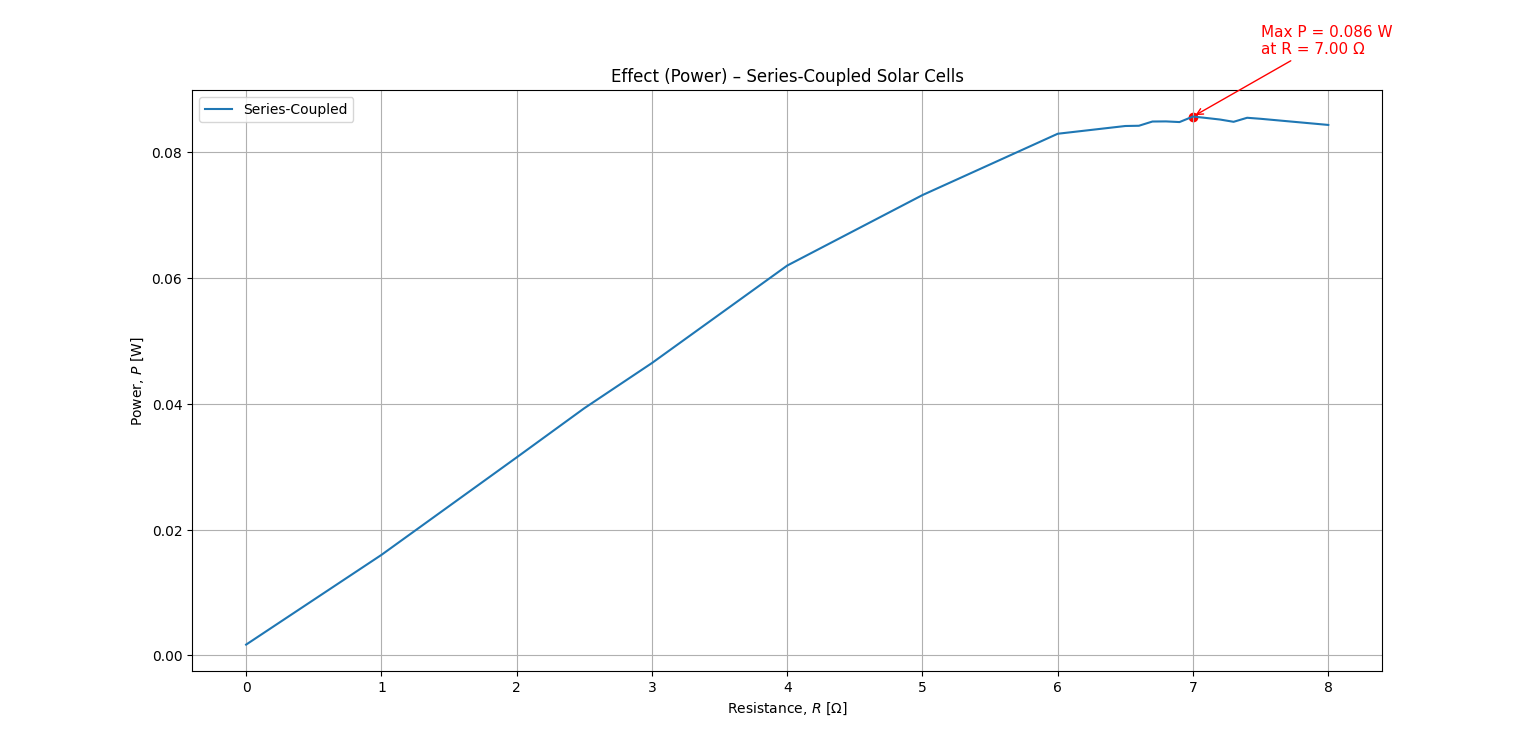
\includegraphics[width=\linewidth]{9.png}
\caption{ Plot of  the effect as a function of resistance for solar cells connected in series   }
\label{fig:9}
\end{figure}
The maximum output of the power P is \( 0.086 \pm 0.009\)W corresponds to resistance \( R = 7 \pm 0.35\Omega \).
\newline
\textbf{Part B }: solar cells connected in parallel. 
The measurements obtained for this
configuration are shown in the table \ref{tab:cell_parallel}

\begin{table}[H]
\centering
\begin{tabular}{|c|c|c|}
\hline
\textbf{I\(\pm 0.05\%\) (mA)} & \textbf{V\(\pm0.025\%\) (V)} & \textbf{R \(\pm0.05\%\) ($\Omega$)} \\
\hline
0.264 & 0.038 & 0.0  \\
0.252 & 0.278 & 1.0  \\
0.246 & 0.319 & 1.2  \\
0.232 & 0.370 & 1.5  \\
0.227 & 0.384 & 1.6  \\
0.220 & 0.395 & 1.7  \\
0.215 & 0.405 & 1.8  \\
0.208 & 0.414 & 1.9  \\
0.200 & 0.421 & 2.0  \\
0.171 & 0.445 & 2.5  \\
0.148 & 0.457 & 3.0  \\
\hline
\end{tabular}
\caption{Measured current, voltage, and resistance values for solar cell connected in parallel .}
\label{tab:cell_parallel}
\end{table}


Plotting these values to obtain the P-R curve for parallel connected solar cells as shown in figure  \ref{fig:10}:

\begin{figure}[hbt!]
    \center
    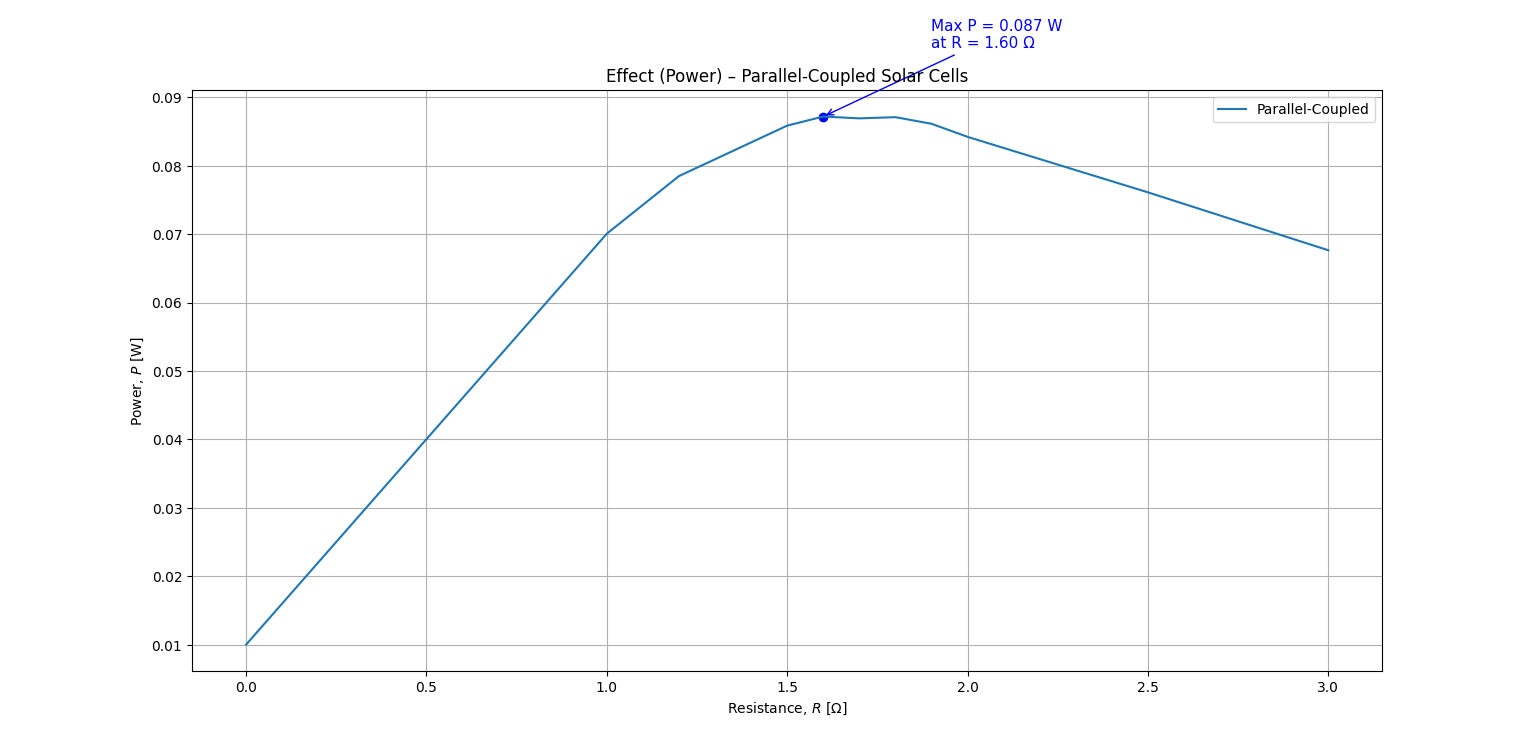
\includegraphics[width=\linewidth]{10.png}
\caption{ Plot of  the effect as a function of resistance for solar cells connected in parallel.   }
\label{fig:10}
\end{figure}
The maximum output of the power P is \( 0.087 \pm 0.009\)W corresponds to resistance \( R = 1.6 \pm 0.08 \Omega \).
\newline

A good way to compare the curves of parallel-connected and series-connected solar cells is to plot both curves in the  same graph as shown in figure \ref{fig:11}:

\begin{figure}[H]
    \center
    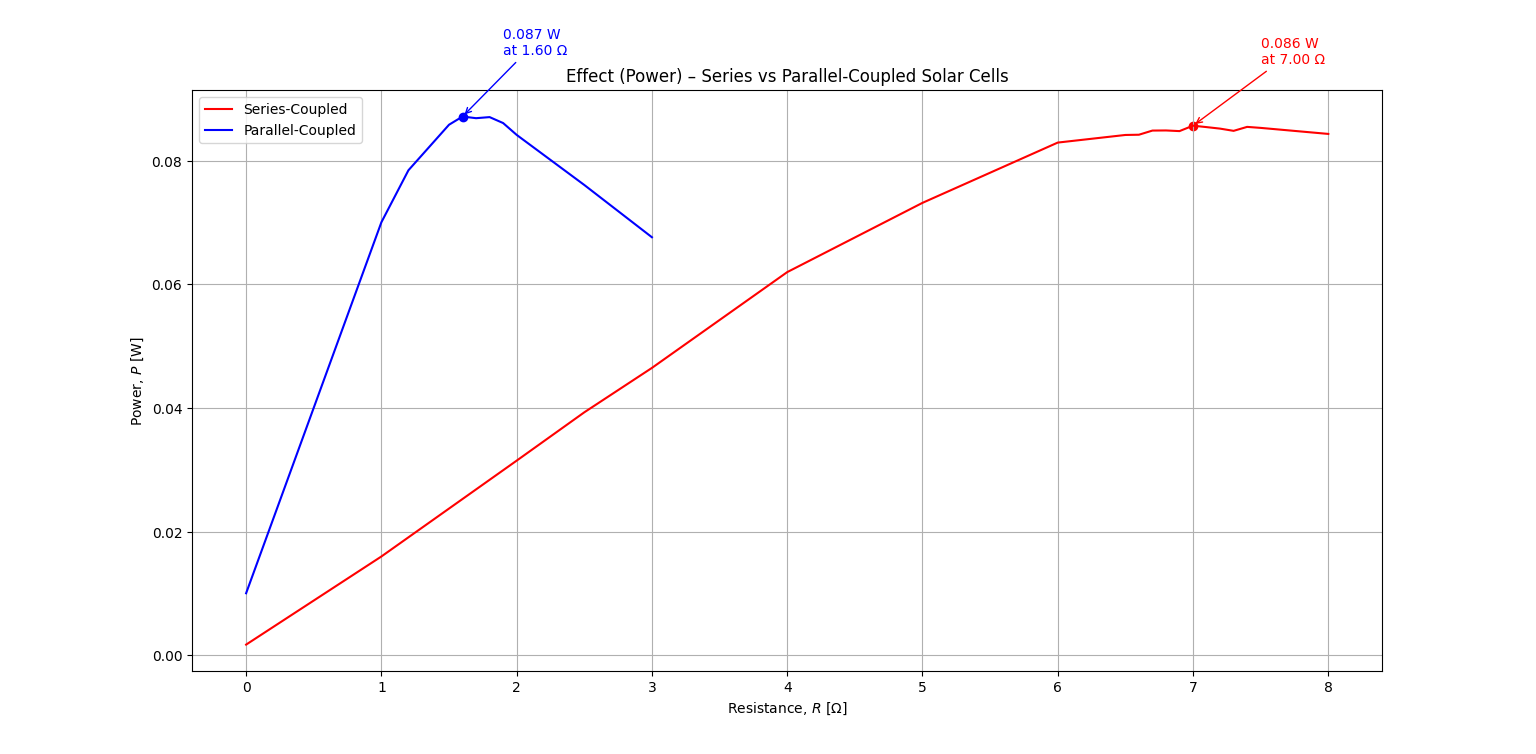
\includegraphics[width=\linewidth]{11.png}
\caption{ P-R curve for parallel-connected compared to  series-connected  solar cells }
\label{fig:11}
\end{figure} 

\subsection{Non-Uniformly illumination}
\textbf{Part A }:  In this part, we measure the current \textbf{I} and voltage \textbf{V}  for different values of resistance \textbf{R} of series-connected solar cells while simulating shading by partially covering one of the solar cells. The results are presented in the table \ref{tab:series_shading}  below

\begin{table}[H]
\centering
\begin{tabular}{|c|c|c|}
\hline
\textbf{I\(\pm 0.05\%\) (mA)} & \textbf{V \(\pm0.025\)(V)} & \textbf{R \(\pm0.05\%\)($\Omega$)} \\
\hline
0.036 & 0.040 & 0.0   \\
0.036 & 0.038 & 1.0   \\
0.036 & 0.074 & 2.0   \\
0.036 & 0.110 & 3.0   \\
0.036 & 0.145 & 4.0   \\
0.036 & 0.181 & 5.0   \\
0.036 & 0.217 & 6.0   \\
0.035 & 0.252 & 7.0   \\
0.035 & 0.287 & 8.0   \\
0.035 & 0.322 & 9.0   \\
0.035 & 0.357 & 10.0  \\
0.035 & 0.532 & 15.0  \\
0.033 & 0.677 & 20.0  \\
0.033 & 0.700 & 21.0  \\
0.032 & 0.720 & 22.0  \\
0.031 & 0.736 & 23.0  \\
0.031 & 0.752 & 24.0  \\
0.030 & 0.760 & 24.5  \\
0.030 & 0.767 & 25.0  \\
0.030 & 0.772 & 25.5  \\
0.030 & 0.778 & 26.0  \\
0.029 & 0.790 & 27.0  \\
0.027 & 0.816 & 30.0  \\
\hline
\end{tabular}
\caption{Measured current, voltage, and resistance values for series-connected solar cells under partial shading.}
\label{tab:series_shading}
\end{table}

Plotting these values to obtain the P-R curve for series- connected solar cells in simulated shading  as shown in figure \ref{fig:12}:

\begin{figure}[H]
    \center
    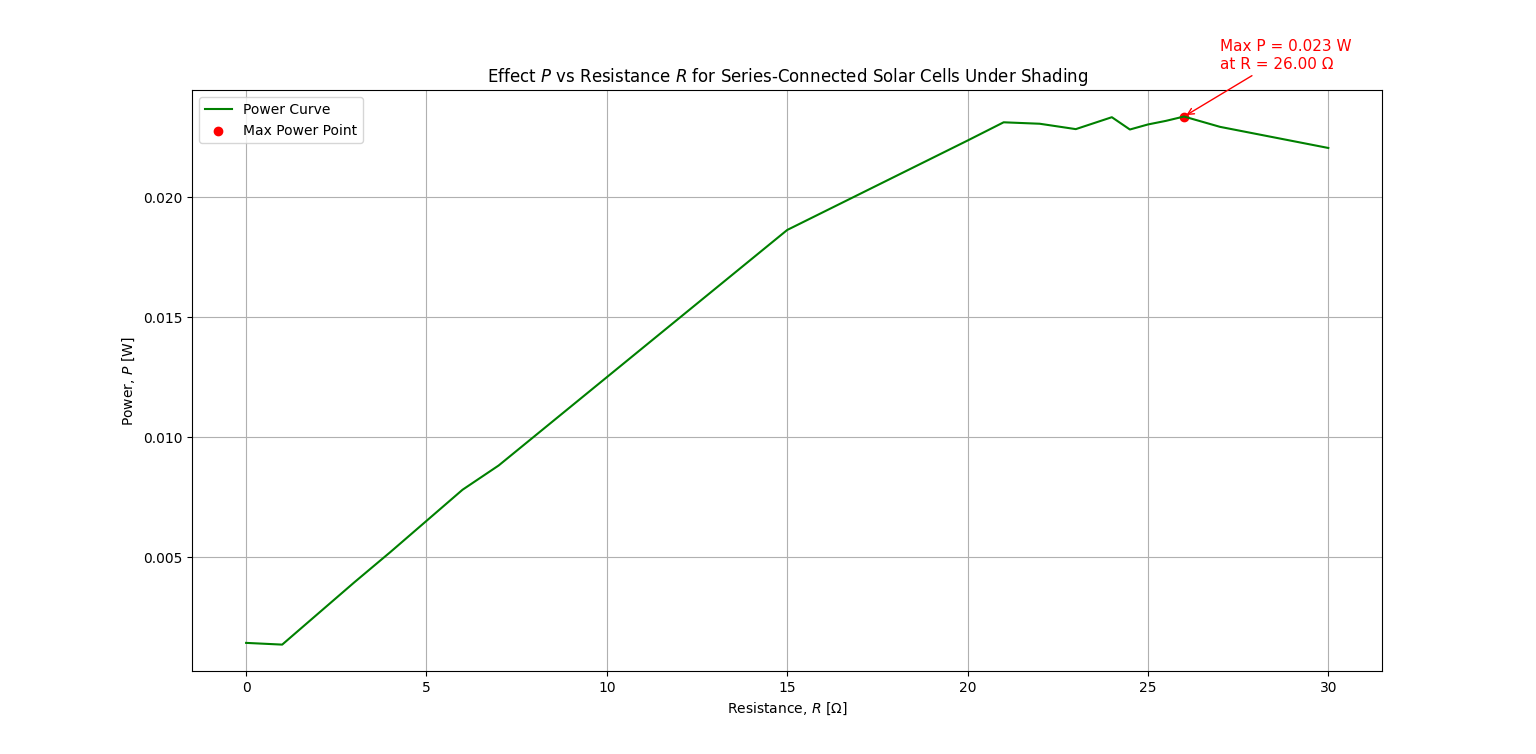
\includegraphics[width=\linewidth]{12.png}
\caption{ P-R curve for series-connected   solar cells in partially shading  }
\label{fig:12}
\end{figure} 
The maximum output of the power P is \( 0.023 \pm 0.003\)W corresponds to resistance \( R = 26\pm 1.3 \Omega \).










\textbf{Part B }:  In this part, we measure the current \textbf{I} and voltage \textbf{V}  for different values of resistance \textbf{R} of parallel-connected solar cells while simulating shading by partially covering one of the solar cells. The results are presented in the table \ref{tab:parallel_shading}  below:

\begin{table}[H]
\centering
\begin{tabular}{|c|c|c|}
\hline
\textbf{I\(\pm0.05\%\) (mA)} & \textbf{V\(\pm0.025\%\) (V)} & \textbf{R\(\pm0.05\%\) ($\Omega$)} \\
\hline
0.176 & 0.022 & 0.0 \\
0.173 & 0.187 & 1.0 \\
0.167 & 0.265 & 1.5 \\
0.157 & 0.327 & 2.0 \\
0.156 & 0.338 & 2.1 \\
0.153 & 0.349 & 2.2 \\
0.150 & 0.358 & 2.3 \\
0.147 & 0.366 & 2.4 \\
0.145 & 0.373 & 2.5 \\
0.142 & 0.381 & 2.6 \\
0.139 & 0.387 & 2.7 \\
0.136 & 0.392 & 2.8 \\
0.133 & 0.396 & 2.9 \\
0.129 & 0.400 & 3.0 \\
0.117 & 0.419 & 3.5 \\
0.106 & 0.431 & 4.0 \\
\hline
\end{tabular}
\caption{Measured current, voltage, and resistance values for parallel-connected solar cells under partial shading.}
\label{tab:parallel_shading}
\end{table}

Plotting these values to obtain the P-R curve for parallel- connected solar cells in simulated shading  as shown in figure \ref{fig:13}:

\begin{figure}[H]
    \center
    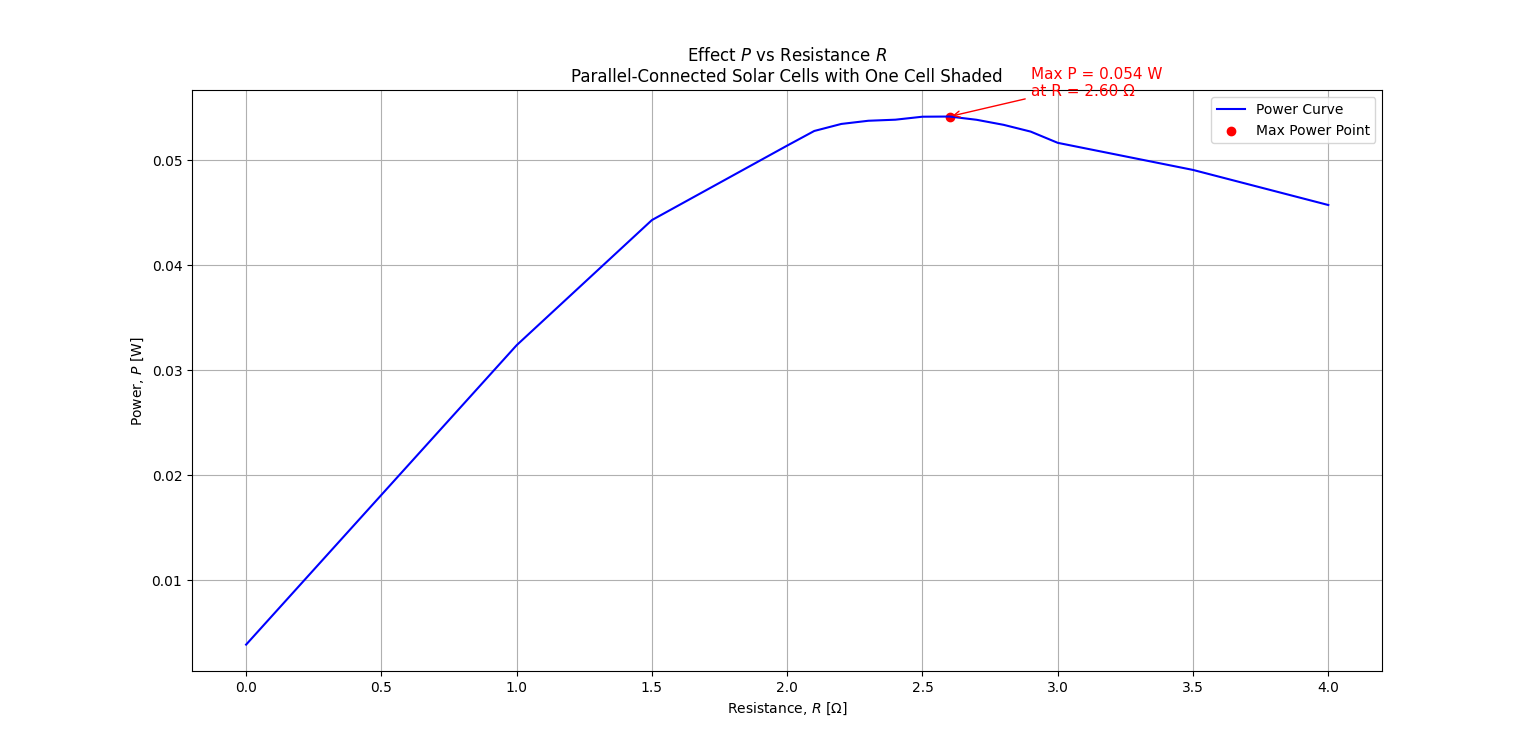
\includegraphics[width=\linewidth]{13.png}
\caption{ P-R curve for parallel-connected   solar cells in partially shading  }
\label{fig:13}
\end{figure} 
The maximum output of the power P is \( 0.054 \pm 0.005\)W corresponds to resistance \( R = 2.6 \pm0.13 \Omega \).




A good way to compare the curves of parallel-connected and series-connected solar cells in partial shading  is to plot both curves in the  same graph as shown in figure \ref{fig:14}:

\begin{figure}[H]
    \center
    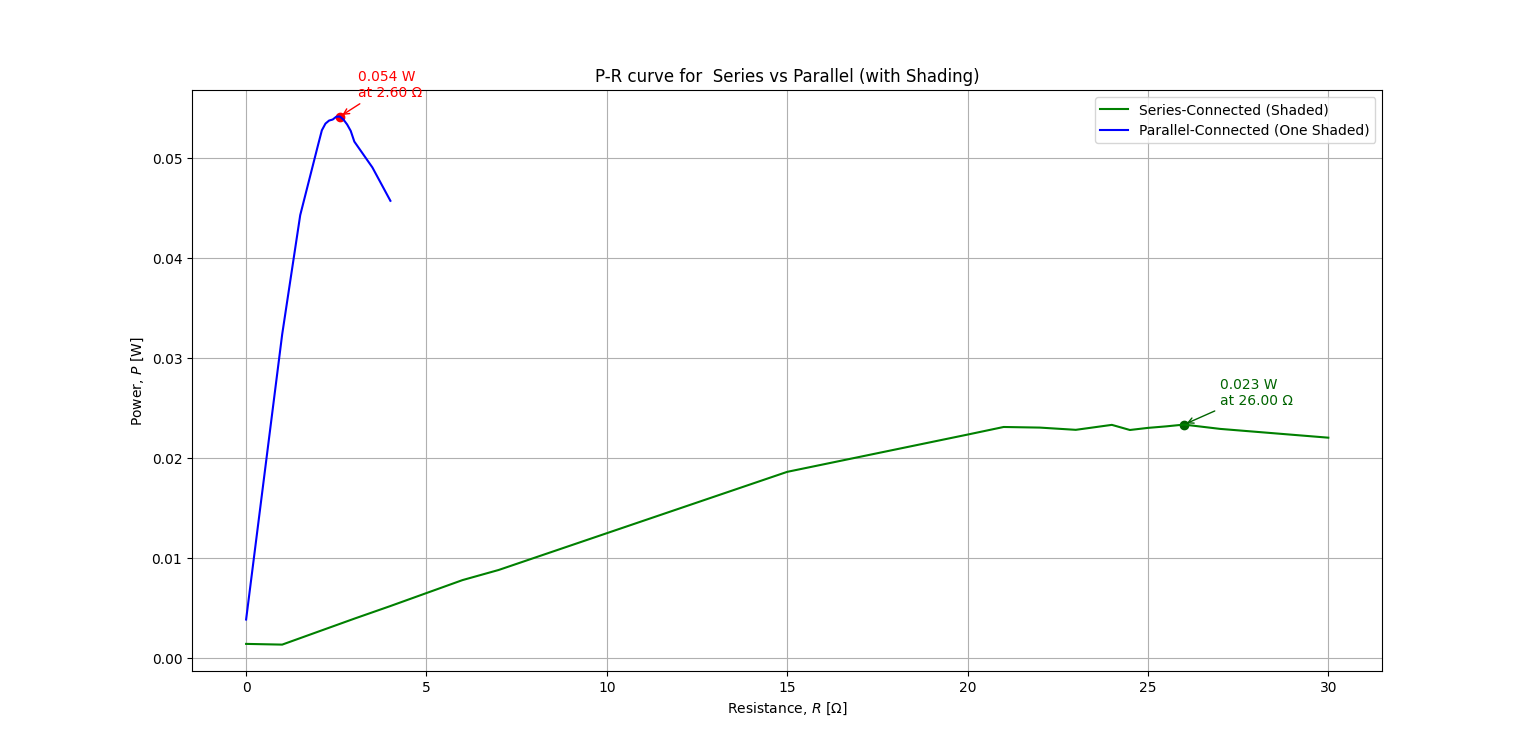
\includegraphics[width=\linewidth]{14.png}
\caption{ P-R curve for parallel-connected compared to  series-connected  solar cells in partial shading }
\label{fig:14}
\end{figure}

\subsection{Discussion }
\subsubsection{The solar cell as a semiconductor
diode}
In this part of the experiment, we measured the current and voltage produced by a single solar cell for both illuminated and dark conditions. We then plotted the experimentally obtained  I–V characteristics to compare with the reference theoretical curve provided in figure\ref{fig:4}

The resulting graph, shown in Figure \ref{fig:7} is close to the reference theoretical curve . 
\newline

\textbf{Near the short-circuit current $(Isc)$:} In this region,the current is mainly determined by the photocurrent generated due to the absorption of light.The current is almost constant, leading to an almost  flat curve.

\textbf{Near the open-circuit voltage $(V_{oc})$:} In this region, the output current is close to zero, and the voltage approaches the open-circuit voltage. As the voltage changes from negative to positive, there is an exponential increase in the current with voltage. This leads to a sharp increase in the curve we see.


\subsubsection{The solar cell’s optimal load}

In this experiment, the resulting graph is shown in Figure \ref{fig:8}.
From the graph, we can observe that the power output of the solar cell depends on the resistance of the connected load. The power increases with resistance, reaching a maximum value of approximately $P\approx 0.043\pm 0.    0055 W$
at around $R\approx 3.2 \pm 0.16\Omega$, which can be considered the optimal load. After this point, the power output begins to decline.


\subsubsection{Combination of single solar cells into a solar panel}

In this experiment, we examined the power output of parallel-connected versus series-connected solar cells.
From Figure \ref{fig:11}, where both curves are plotted on the same graph, we observe the following: the parallel-connected solar cells achieve a maximum power effect of \(P = 0.087 \pm 0.009 \)W when the load is \( R = 1.6 \pm 0.08\Omega \),while the series-connected solar cells reach a maximum effect  of \(P = 0.086\pm0.009 \)W when the load is \( R = 7\pm 0.35 \Omega \).
By comparing the two configurations, we note that parallel-connected solar cells require  lower resistance to reach their maximum power output than series-connected ones .
\newline

In comparison to the single solar cell results shown in Figure \ref{fig:8}, we find that the series configuration produces approximately twice the power of a single cell and does so at double the optimal load \(R = 7\Omega  \) compared to \(R = 3.2\Omega  \) for single cell.


At the same time, the parallel-connected solar cells also produce about twice the power of a single cell, but at half the optimal load \(R = 1.6\Omega \) compared to \(R = 3.2\Omega  \) for single cell.


\textbf{This makes the two-solar-cell configurations, more precisely: parallel-connected solar cells ,  a better option than a single cell in  optimal illumination conditions}

\subsubsection{Non-Uniformly illumination}

In this experiment, we examined the power output of parallel-connected versus series-connected solar cells under non-uniform illumination conditions.

The results are presented in Figure \ref{fig:14}, where both curves are plotted on the same graph. From this graph, we observe that in shading conditions, parallel-connected solar cells produced a maximum power  of \(P= 0.54 \pm 0.005 \text{W} \) at an optimal load of \( R = 2.6 \pm 0.13 \, \Omega \), while series-connected solar cells produced a maximum power  of  \( P=0.23\pm 0.003 \text{W} \) at an optimal load of \( R = 26\pm 1.3 \, \Omega \).

\textbf{This makes the parallel-connected configuration much more efficient than the series-connected configuration under non-uniform illumination.
In fact, it is more effective to use a single solar cell than to connect two cells in series under shading condition }.
\subsubsection{Summery}
% Requires: \usepackage{colortbl}
\begin{table}[H]
    \centering
    \begin{tabular}{|l|c|c|}
    \hline
    & \textbf{Series} & \textbf{Parallel} \\ \hline
    \textbf{Uniform illumination} &\( P = 0.086\pm 0.009 \) W &\( P = 0.087\pm 0.009 \) W \\ \hline
    \textbf{Partial shade} &\(P=  0.23\pm 0.005\)W &\( P=0.54 \pm 0.003 \)W \\ \hline
    \end{tabular}
    \caption{Comparison of Series and Parallel under Different Conditions}
    \label{tab:sum}
\end{table}













\subsection{Conclusion}

In this set of experiments, we investigated the electrical behavior  of solar cells under various conditions. Starting with a single solar cell, we measured current and voltage under both illuminated and dark conditions and in acceptable way reproduced the  characteristic I–V curve, which aligned well with theoretical reference graph .

We then explored how the power output of a solar cell varies with load resistance. The results showed that power increases with resistance up to an optimal value, beyond which it declines. For a single solar cell, the maximum power  achieved  at approximately \( R = 3.2\, \Omega \), producing around \( 0.043 \, \text{W} \).

Next, we compared two solar cells connected in series and in parallel. Under uniform illumination, both configurations produced  nearly twice the power of a single cell, with the series connection requiring approximately \( R = 7 \, \Omega \) and the parallel connection around \( R = 1.6 \, \Omega \) for optimal power output. These results confirm that either configuration can improve performance compared to a single cell. 

Finally,we examined the behavior  under non-uniform illumination (simulating partial shading). 
The parallel-connected solar cells produced a significantly higher maximum power output (\( 0.54 \, \text{W} \) at \( R = 2.6 \, \Omega \)) compared to the series-connected configuration (\( 0.23 \, \text{W} \) at \( R = 26 \, \Omega \)). This shows  the disadvantages of series-connected solar cells in shading conditions and highlights the advantages  of the parallel configuration in such conditions .
In fact, under partial shading, even a single solar cell can be a better option than  two solar cells connected in series.

To summarize : based of the results presented earlier  , we conclude that the parallel-connected solar cells is the optimal option regardless of the illumination conditions .


\begin{thebibliography}{1}

\bibitem{squires}
G.~L. Squires, \emph{Practical Physics}, 4th~ed. Cambridge: Cambridge University Press, 2001.



\bibitem{manual}
Department of Physics, \emph{Datablader-Solcellen}, [UIO], FYS2150 semester Lab Notes , 2025.

\end{thebibliography}




\end{document}

\(  \)
\(  \)
\(  \)
\(  \)
\(  \)
\(  \)
\begin{itemize}
    \item  Part A: When the solar cell is exposed to light  .
    \item  Part B: :When the solar cell is in darkness. 
\end{itemize}



\begin{figure}[h]
    \center
    \includegraphics[width=\linewidth]{.png}
\caption{   }
\label{fig:}
\end{figure}



\ref{fig:11}:

\begin{figure}[hbt!]
    \center
    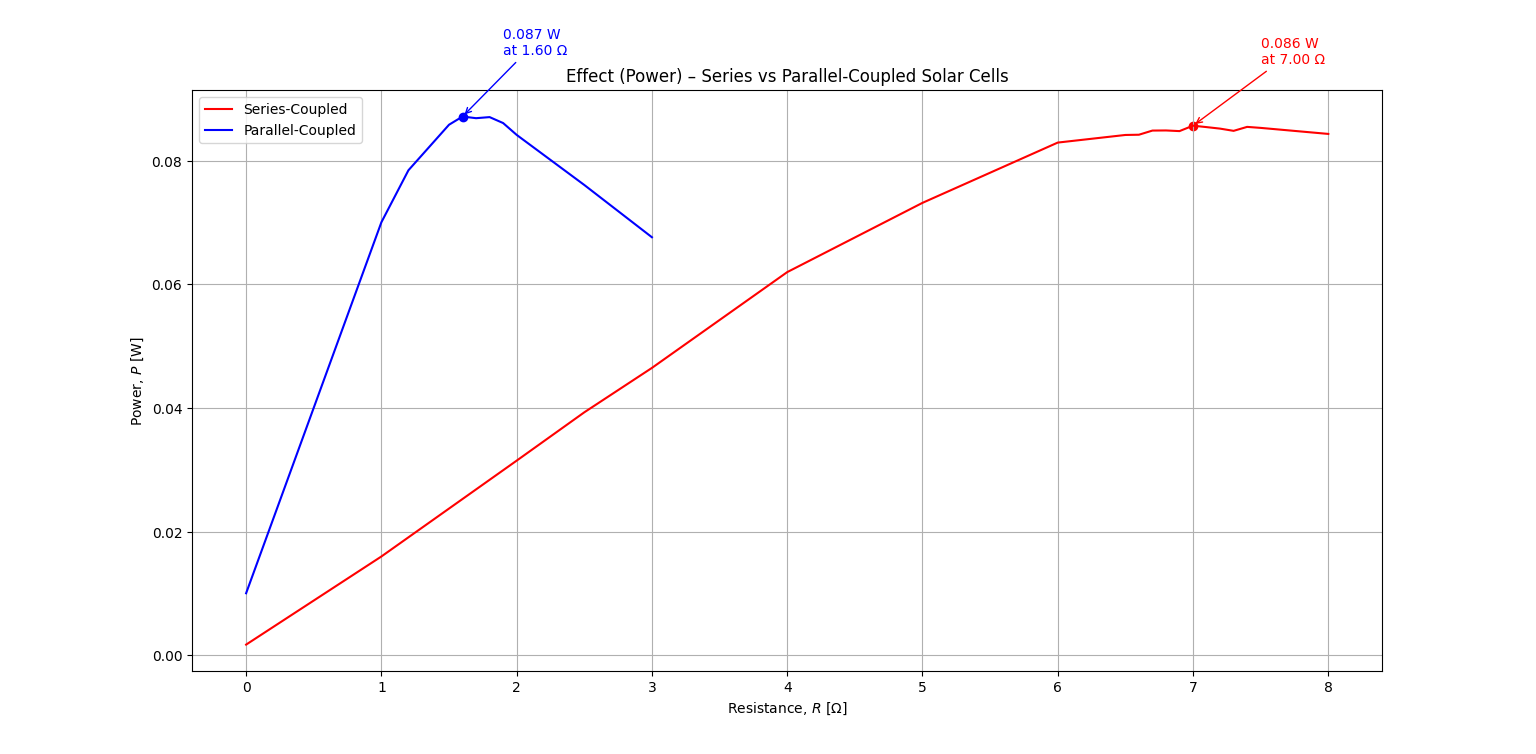
\includegraphics[width=\linewidth]{11.png}
\caption{ P-R curve for parallel-connected compared to  series-connected  solar cells }
\label{fig:11}
\end{figure} 
